%https://www.overleaf.com/learn/latex/Creating_a_document_in_LaTeX
%https://oeis.org/wiki/List_of_LaTeX_mathematical_symbols
\documentclass[12pt]{report}
\usepackage{graphicx}
\graphicspath{ {./../Output/} {./../} }

\title{CS 440: Probabilistic Search}
\author{Steven Nguyen \& Kyra Kennedy}
\date{10 April 2021}

\begin{document}

\begin{titlepage}
\maketitle
\end{titlepage}

\section*{Abstract}
In this project, we demonstrated basic techniques of supervised learning and computer vision in Python.

\section*{Academic Integrity}
-

\section*{The Basic Coloring Agent}
\begin{figure}
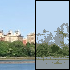
\includegraphics[width=.5\textwidth]{Basic Agent Prediction}
\caption{In the above picture, the left is the training data and the right is the prediction}
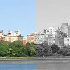
\includegraphics[width=.5\textwidth]{Test Image}
\caption{In the above picture, the left is the training data and the right is the test data}
\end{figure}
The final result isn't great. Though it has the water, sky, and tree colors correctly placed, there many problems. The main problems were that we used 5 k-means, so we can only have 5 of the many colors; because we used patches of 3x3, we can't color the edge of the image; and because we only used 3x3 patches, each test pixel does not have that much information to work off of.\\
We could measure the quality of the final result using P-Norms between the actual image and the prediction. We implemented checking the L2 Norm in Agent.check\_prediction(). This prediction is somewhat numerically satisfying, but still, not great.

\section*{The Improved Coloring Agent}
\begin{figure}
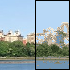
\includegraphics[width=.5\textwidth]{Improved Agent Prediction}
\caption{In the above picture, the left is the training data and the right is the prediction}
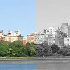
\includegraphics[width=.5\textwidth]{Test Image}
\caption{In the above picture, the left is the training data and the right is the test data}
\end{figure}
The improved agent, or Color M.E. Happy (Mesmerizing Execution), functions in a similar way to the basic agent. To improve this agent, more color clusters (10 instead of 5) were considered and 5x5 clusters were used so the agent could have greater accuracery in choosing colors.\\
One of the reasons a linear model is a bad idea for colorizing an image is the fact that the data isn't really linear, and shouldn't be treated as such. Since each pixel, in the end, has to be represented by three separate values (RGB), a linear model can't accurately expresses how all three of these values interact and ultimately affect the final image.\\
Ideally, with all the time, energy, and resources, the improved agent could use a strong parametric model that adjusts what color is chosen based, not only on the training data, but related pixels in the image being processed so the final result is more comprehensive. Neural networks, as proposed in the project description, could also be used to provide deeper training.

\end{document}